Identifying hidden communities within networks is a crucial graph analytics problem that arises in various domains such as drug discovery, disease prediction, protein annotation, topic discovery, inferring land use, and criminal identification. Here, we want to identify groups of vertices that exhibit dense internal connections but sparse connections with the rest of the graph. One of the difficulties in the community detection problem is the lack of apriori knowledge on the number and size distribution of communities. These communities are intrinsic when identified based on network topology alone, without external attributes, and they are disjoint when each vertex belongs to only one community \cite{com-gregory10}. However, the problem is NP-hard, and there is a lack of apriori knowledge on the number and size distribution of communities \cite{com-blondel08}. To solve this issue, researchers have come up with a number of heuristics for finding communities \cite{com-guimera05, com-derenyi05, com-newman06, com-reichardt06, com-raghavan07, com-blondel08, com-rosvall08, infomap-rosvall09, com-fortunato10, com-gregory10, com-kloster14, com-come15, com-ruan15, com-newman16, com-ghoshal19, com-rita20, com-lu20, com-gupta22}. To measure the quality of communities identified, fitness metrics such as the modularity score proposed by Newman et al. \cite{com-newman06} are used.\ignore{Normalized Mutual Information index (NMI) \cite{com-jain17, com-chopade17}, and Jaccard Index \cite{com-jain17} are also employed.}

The \textit{Louvain method}, proposed by Blondel et al. \cite{com-blondel08}, is one of the most popular community detection algorithms \cite{com-lancichinetti09}. It is a greedy, modularity-based optimization algorithm, that hierarchically agglomerates vertices in a graph to obtain communities \cite{com-blondel08}. It has a time complexity of $O(KM)$\ignore{and an average time complexity of $\Theta (N \log N)$} (where $M$ represents the number of edges in the graph, $K$ the total number of iterations performed across all passes), and it efficiently identifies communities with resulting high modularity. A number of algorithmic improvements to the Louvain algorithm have been proposed \cite{com-rotta11, com-waltman13, com-gach14, com-ryu16, com-ozaki16, com-traag15, com-lu15, com-naim17, com-halappanavar17, com-ghosh18, com-traag19, com-shi21, com-zhang21, com-you22, com-aldabobi22}. To parallelize the algorithm on multicore CPUs \cite{staudt2015engineering, staudt2016networkit, com-fazlali17, com-halappanavar17, qie2022isolate}, GPUs \cite{com-naim17}, CPU-GPU hybrids \cite{com-bhowmik19, com-mohammadi20}, multi-GPUs \cite{com-cheong13, hricik2020using, chou2022batched, com-gawande22}, and multi-node systems \cite{com-ghosh18, ghosh2018scalable, sattar2022scalable, com-bhowmick22}, a number of strategies have been attempted \cite{com-cheong13, com-wickramaarachchi14, com-zeng15, com-que15, com-fazlali17, com-naim17, com-halappanavar17, com-ghosh18, com-bhowmik19, com-mohammadi20, com-shi21, com-bhowmick22}.

However, many real-world graphs rapidly evolve with time, through the insertion/deletion of edges/vertices. These graphs are usually immense in scale, stemming from applications such as machine learning and social networks, and are gradually becoming ubiquitous.\ignore{With this data deluge, newer challenges are emerging.} For efficiency reasons, one needs algorithms that update the results without re-computing from scratch. Such algorithms are known as \textit{dynamic algorithms}. Parallel algorithms for graph analytics on dynamic graphs have thus become a subject of considerable research interest. Examples of parallel dynamic algorithms include those for dynamic graph coloring \cite{color-yuan17, color-bhattacharya18}, maintaining shortest routes \cite{path-zhang17, path-khanda21}, and updating centrality scores \cite{cent-shao20, cent-regunta21}.

A growing number of research efforts have focused on detecting communities in dynamic networks. The goal of dynamic community detection is to obtain high-quality communities while minimizing computation time. A suitable dynamic community detection approach should find an approximate affected set of vertices that covers most of the true affected set of vertices as possible (too small and we get bad communities, too large and we increase computation time), while requiring the least amount of time (overhead) \cite{incr-ramalingam96}. Note that if the subset of the graph identified as \textit{affected} is too small, we may end up with inaccurate communities, and if the subset is too large, we incur a significant computation time. Hence, one should look to identify the appropriate set of affected vertices. In addition, determining the vertices to be processed should have low overhead \cite{incr-ramalingam96}.

\ignore{The simplest approach for dynamic community detection is to use the community membership of vertices from the previous snapshot of the graph \cite{com-aynaud10, com-chong13, com-shang14, com-zhuang19} (which we call \textit{Naive-dynamic}). Alternatively, more advanced techniques have been employed to minimize computation by identifying a smaller subset of the graph that is affected by changes, such as moving only changed vertices \cite{com-aktunc15, com-yin16}, recomputing vertices close to an updated edge (below a given threshold distance) \cite{com-held16}, disbanding affected communities to lower-level network \cite{com-cordeiro16}, or using a dynamic modularity metric to compute community membership of vertices from scratch \cite{com-meng16}. \textit{Delta-Screening} (or \textit{$\Delta$-screening}) is a recently proposed technique that finds a subset of vertices impacted by changes in a graph using delta-modularity \cite{com-zarayeneh21}.}

However, a critical examination of the extant literature on dynamic community detection algorithms indicates a few shortcomings. Some of these algorithms \cite{com-cordeiro16, com-meng16} do not outperform static algorithms even for modest-sized batch updates. Aynaud et al. \cite{com-aynaud10} and Chong et al. \cite{com-chong13} adapt the existing community labels and run an algorithm, such as Louvain, on the entire graph. Often, this is unwarranted since not every vertex would need to change its community on the insertion/deletion of a few edges. Cordeiro et al. \cite{com-cordeiro16} do not consider the cascading impact of changes in community labels, where the community label of a vertex changes because of a change in the community label of its neighbor. Zarayeneh et al. \cite{com-zarayeneh21} identify a subset of vertices whose community labels are likely to change on the insertion/deletion of a few edges. However, as this set of vertices identified is large, the algorithm of Zaranayeh et al. incurs a significant computation time. Moreover, most of the reported algorithms \cite{com-aynaud10, com-chong13, com-meng16, com-cordeiro16, com-zhuang19, com-zarayeneh21} are sequential. There is thus a pressing need for efficient parallel algorithms for community detection on large dynamic graphs. Further, none of the works recommend reusing the previous \textit{total edge weight} of each vertex/community (required for local-moving phase of Louvain algorithm) as auxiliary information to the dynamic algorithm. Recomputing it from scratch is expensive and becomes a bottleneck for dynamic Louvain algorithm. Table \ref{tab:compare} summarizes the above discussion.

\begin{table}[hbtp]
  \centering
  \caption{Speedup of our multicore implementation of Leiden algorithm compared to other state-of-the-art implementations. Direct comparisons entail running the given implementation on our server, while indirect comparisons (marked with a $*$, explained in Section \ref{sec:comparison-indirect}) involve comparing results relative to a common reference\ignore{(original Leiden)}.\ignore{Notably, the Leiden implementations vary in their classification, with some being multi-core and others multi-node.}}
  \label{tab:compare}
  \begin{tabular}{|c|c||c|}
    \toprule
    \textbf{Leiden implementation} &
    \textbf{Published} &
    \textbf{Our Speedup} \\
    \midrule
    Static \cite{sahu2023gvelouvain} & 2023 & $22\times$ \\ \hline
    Naive-dynamic \cite{csardi2006igraph} & 2006 & $\gg 50\times$ \\ \hline
    Delta-screening \cite{com-zarayeneh21} & 2021 & $\gg 20\times$ \\ \hline
    DynaMo \cite{com-zhuang19} & 2019 & $\gg 166\times^*$ \\ \hline
    Batch \cite{com-chong13} & 2013 & $\gg 22\times^*$ \\ \hline
  \bottomrule
  \end{tabular}
\end{table}





\subsection{Our Contributions}

This paper addresses the design of an efficient Parallel Louvain algorithm in the batch dynamic setting, where multiple edge updates are processed simultaneously. We first discuss our Dynamic Frontier (DF) approach that incrementally identifies an approximate set of affected vertices in the graph, given a batch of edge deletions and insertions, with low runtime overhead. In addition to accepting the previous community membership of each vertex, our algorithm accepts the previous total edge weight of each vertex as auxiliary information in order to improve scalability. We then show how to combine our DF approach with the Louvain method. We compare DF with two other dynamic approaches, the Naive-dynamic (ND) approach, and the $\Delta$-screening ($\Delta S$) approach. On a collection of $12$ graphs from four different classes, our experiments indicate that DF Louvain has a mean improved performance of $1.5\times$ compared to ND Louvain, while obtaining communities of the same quality. The work presented by Zarayeneh et al. \cite{com-zarayeneh21} demonstrates improved performance of $\Delta$-screening compared to Dynamo \cite{com-zhuang19} and Batch \cite{com-chong13}. As the DF approach outperforms $\Delta$-screening, we expect similar gains compared to Dynamo and Batch. Further, unlike Static Louvain, which may change significantly the way communities are obtained between snapshots (two runs in the snapshot lead to different solutions due its non-determinism), in our proposed algorithm, unaffected communities keep unchanged, i.e., they preserve the same nodes and even the same community id between snapshots. Community stability is important because it will simplify the process of tracking of communities over time. We show that our algorithm achieves \textit{good} community stability. Finally, we show that our algorithm has good scaling performance.




%% - Use --- for a dash.
%% - Use ``camera-ready'' for quotes.
%% - Use {\itshape very} or \textit{very} for italicized text.
%% - Use \verb|acmart| or {\verb|acmart|} for mono-spaced text.
%% - Use \url{https://capitalizemytitle.com/} for URLs.
%% - Use {\bfseries Do not modify this document.} for important boldface details.
%% - Use \ref{fig:name} for referencing.

%% For a block of pre-formatted text: 
% \begin{verbatim}
%   \renewcommand{\shortauthors}{McCartney, et al.}
% \end{verbatim}

%% For a list of items:
% \begin{itemize}
% \item the ``ACM Reference Format'' text on the first page.
% \item the ``rights management'' text on the first page.
% \item the conference information in the page header(s).
% \end{itemize}

%% For a table:
% \begin{table}
%   \caption{Frequency of Special Characters}
%   \label{tab:freq}
%   \begin{tabular}{ccl}
%     \toprule
%     Non-English or Math&Frequency&Comments\\
%     \midrule
%     \O & 1 in 1,000& For Swedish names\\
%     $\pi$ & 1 in 5& Common in math\\
%     \$ & 4 in 5 & Used in business\\
%     $\Psi^2_1$ & 1 in 40,000& Unexplained usage\\
%   \bottomrule
% \end{tabular}
% \end{table}

%% For a full-width table:
% \begin{table*}
%   \caption{Some Typical Commands}
%   \label{tab:commands}
%   \begin{tabular}{ccl}
%     \toprule
%     Command &A Number & Comments\\
%     \midrule
%     \texttt{{\char'134}author} & 100& Author \\
%     \texttt{{\char'134}table}& 300 & For tables\\
%     \texttt{{\char'134}table*}& 400& For wider tables\\
%     \bottomrule
%   \end{tabular}
% \end{table*}


%% For inline math:
% \begin{math}
%   \lim_{n\rightarrow \infty}x=0
% \end{math},

%% For a numbered equation:
% \begin{equation}
%   \lim_{n\rightarrow \infty}x=0
% \end{equation}

%% For an unnumbered equation:
% \begin{displaymath}
%   \sum_{i=0}^{\infty} x + 1
% \end{displaymath}

%% For a figure:
% \begin{figure}[h]
%   \centering
%   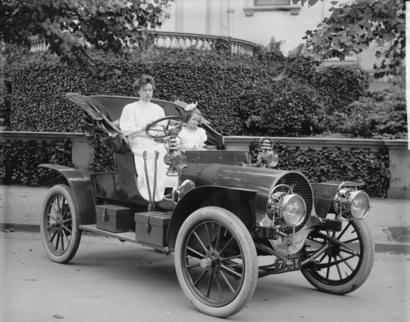
\includegraphics[width=\linewidth]{inc/sample-franklin}
%   \caption{1907 Franklin Model D roadster. Photograph by Harris \&
%     Ewing, Inc. [Public domain], via Wikimedia
%     Commons. (\url{https://goo.gl/VLCRBB}).}
%   \Description{A woman and a girl in white dresses sit in an open car.}
% \end{figure}

%% For a teaser figure.
% \begin{teaserfigure}
%   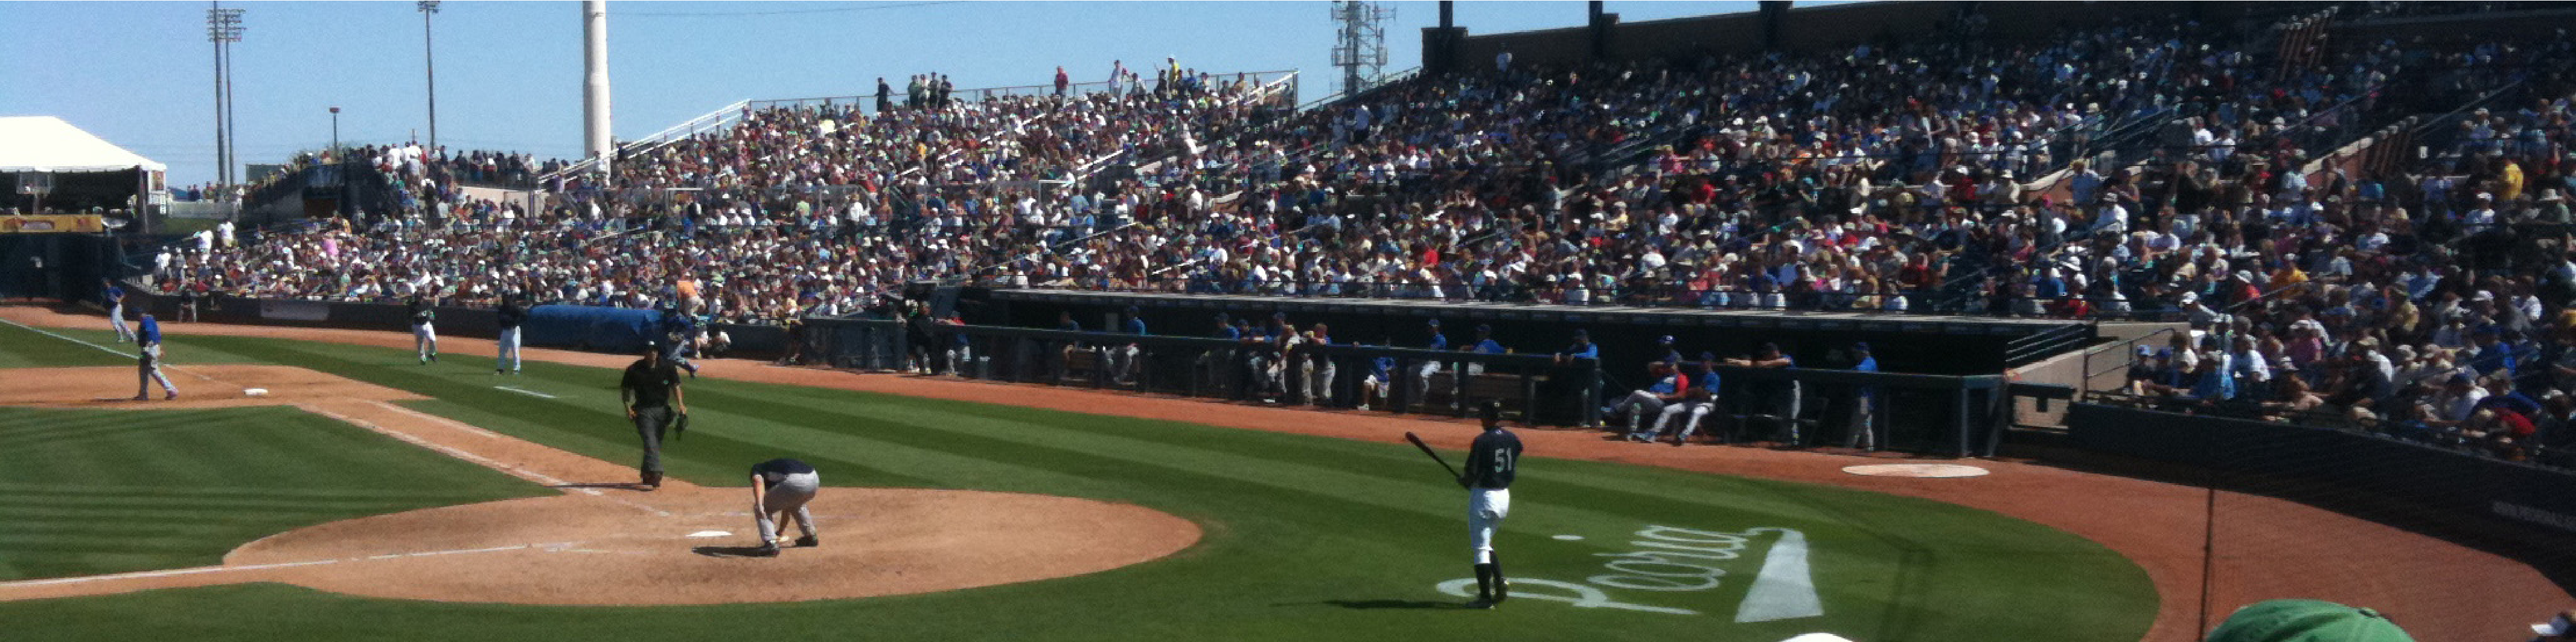
\includegraphics[width=\textwidth]{sampleteaser}
%   \caption{figure caption}
%   \Description{figure description}
% \end{teaserfigure}
